\documentclass[12pt, a4paper, twoside]{scrartcl}
 %---- Allgemeine Layout Einstellungen ------------------------------------------

% Für Kopf und Fußzeilen, siehe auch KOMA-Skript Doku
\usepackage[komastyle]{scrpage2}
\pagestyle{scrheadings}
\setheadsepline{0.5pt}[\color{black}]


%Einstellungen für Figuren- und Tabellenbeschriftungen
\setkomafont{captionlabel}{\sffamily\bfseries}
\setcapindent{0em}


%---- Weitere Pakete -----------------------------------------------------------
% Die Pakete sind alle in der TeX Live Distribution enthalten. Wichtige Adressen
% www.ctan.org, www.dante.de

% Sprachunterstützung
\usepackage[ngerman]{babel}

% Benutzung von Umlauten direkt im Text
% entweder "latin1" oder "utf8"
\usepackage[utf8]{inputenc}

% Pakete mit Mathesymbolen und zur Beseitigung von Schwächen der Mathe-Umgebung
\usepackage{latexsym,exscale,stmaryrd,amssymb,amsmath}

% Weitere Symbole
\usepackage[nointegrals]{wasysym}
\usepackage{eurosym}

% Anderes Literaturverzeichnisformat
%\usepackage[square,sort&compress]{natbib}

% Für Farbe
\usepackage{color}

% Zur Graphikausgabe
%Beipiel: \includegraphics[width=\textwidth]{grafik.png}
\usepackage{graphicx}

% Text umfließt Graphiken und Tabellen
% Beispiel:
% \begin{wrapfigure}[Zeilenanzahl]{"l" oder "r"}{breite}
%   \centering
%   \includegraphics[width=...]{grafik}
%   \caption{Beschriftung} 
%   \label{fig:grafik}
% \end{wrapfigure}
\usepackage{wrapfig}

% Mehrere Abbildungen nebeneinander
% Beispiel:
% \begin{figure}[htb]
%   \centering
%   \subfigure[Beschriftung 1\label{fig:label1}]
%   {\includegraphics[width=0.49\textwidth]{grafik1}}
%   \hfill
%   \subfigure[Beschriftung 2\label{fig:label2}]
%   {\includegraphics[width=0.49\textwidth]{grafik2}}
%   \caption{Beschriftung allgemein}
%   \label{fig:label-gesamt}
% \end{figure}
\usepackage{subfigure}

% Caption neben Abbildung
% Beispiel:
% \sidecaptionvpos{figure}{"c" oder "t" oder "b"}
% \begin{SCfigure}[rel. Breite (normalerweise = 1)][hbt]
%   \centering
%   \includegraphics[width=0.5\textwidth]{grafik.png}
%   \caption{Beschreibung}
%   \label{fig:}
% \end{SCfigure}
\usepackage{sidecap}
\usepackage{float}

% Befehl für "Entspricht"-Zeichen
\newcommand{\corresponds}{\ensuremath{\mathrel{\widehat{=}}}}
\newcommand{\folgt}{\ensuremath{\mathrel{\Rightarrow}}}
\newcommand{\equals}{\ensuremath{\mathrel{\Leftrightarrow}}}
\newcommand{\degree}{\ensuremath{\mathrel{^{\circ}}}}

\newcommand{\nn}{\nonumber}
\newcommand{\tn}[1]{\textnormal{#1}}
\newcommand{\D}{\ensuremath{\mathrel{\rm d}}}

\newcommand{\const}{\tn{const}}

\newcommand{\meter}{\ensuremath{\mathrel{\tn m}}}
\newcommand{\kilogramm}{\ensuremath{\mathrel{\tn{kg}}}}
\newcommand{\second}{\ensuremath{\mathrel{\tn s}}}
\newcommand{\sekunde}{\second}

\newcommand{\volt}{\ensuremath{\mathrel{\tn V}}}
\newcommand{\pascal}{\ensuremath{\mathrel{\tn{Pa}}}}
\newcommand{\coulomb}{\ensuremath{\mathrel{\tn C}}}
\newcommand{\newton}{\ensuremath{\mathrel{\tn N}}}
\newcommand{\liter}{\ensuremath{\mathrel{\tn l}}}
\newcommand{\celsius}{\ensuremath{\mathrel{\tn C}}}
\newcommand{\fahrenheit}{\ensuremath{\mathrel{\tn F}}}
\newcommand{\joule}{\ensuremath{\mathrel{\tn J}}}
\newcommand{\kelvin}{\ensuremath{\mathrel{\tn K}}}
\newcommand{\mol}{\ensuremath{\mathrel{\tn{mol}}}}
\newcommand{\gramm}{\ensuremath{\mathrel{\tn{g}}}}

\newcommand{\kilo}{\ensuremath{\mathrel{\tn k}}}
\newcommand{\hecto}{\ensuremath{\mathrel{\tn h}}}

\newcommand{\centi}{\ensuremath{\mathrel{ \tn c}}}
\newcommand{\milli}{\ensuremath{\mathrel{ \tn m}}}
\newcommand{\micro}{\ensuremath{\mathrel{ \tn\mu }}}



%\newcommand{}{\ensuremath{\mathrel{  }}}
%\newcommand{}{\ensuremath{\mathrel{  }}}
%\newcommand{}{\ensuremath{\mathrel{  }}}


\newcommand{\person}[1]{\textsc{#1}}




 \begin{document}
 %Titelseite
\begin{titlepage}
\centering
\textsc{\Large Anfängerpraktikum der Fakultät für
  Physik,\\[1.5ex] Universität Göttingen}

\vspace*{4.2cm}

\rule{\textwidth}{1pt}\\[0.5cm]
{\huge \bfseries
  Spezifische Wärme der Luft und Gasthermometer}\\[0.5cm]
\rule{\textwidth}{1pt}

\vspace*{3.5cm}

\begin{Large}
\begin{tabular}{ll}
Praktikanten: &  Silke Andrea Teepe\\
& Marcel Kramer\\
E-Mail: & \\
Betreuer: & Alexander Schmelev\\
\end{tabular}
\end{Large}

\vspace*{0.8cm}

\begin{Large}
\fbox{
  \begin{minipage}[t][2.5cm][t]{6cm} 
    Testat:
  \end{minipage}
}
\end{Large}

\end{titlepage}
\cleardoublepage
\tableofcontents
\cleardoublepage
\setcounter{page}{1}

\section{Einleitung}
\label{sec:einleitung}

Tropft man Tinte in ein mit Wasser gefülltes Glas kann man beobachten, wie sich die Farbe im Wasser ausbreitet, bis sie gleichmäßig verteilt ist. Derselbe Effekt tritt auch bei Gasen auf, wie man sich durch öffnen einer Flasche mit einer intensiv riechenden Substanz wie zum Beispiel Parfüm in einem geschlossenen Raum verdeutlichen kann. Dieses selbstständige Durchmischen von Molekülen in Gasen und Flüssigkeiten wird Diffusion genannt und soll in diesem Versuch untersucht werden.

\section{Theorie}
\label{sec:theorie}

\subsection{Die Fickschen Gesetze}

Grundlage der Diffusion ist die Bewegung einzelner Teilchen in Gasen oder Flüssigkeiten. Diese Bewegung von Molekülen in einer Flüssigkeit oder einem Gas wird Braunsche Bewegung genannt. Sie wird durch Stöße verursacht und ist unregelmäßig. Aufgrund der hohen betrachteten Teilchenzahl kann die Bewegungsrichtung der Teilchen nach einem Stoß als gleichverteilt angenommen werden. Die Verteilung der Teilchen im Gas/Wasser soll durch $n(x)$ beschrieben werden. Aus einem Gebiet $A$ mit einer höheren Teilchendichte als in der Umgebung von $A$ werden zunächst also mehr Teilchen aus $A$ hinausgestoßen als von der Umgebung in $A$ hinein gestoßen werden. Sobald die Teilchendichte in beiden Bereichen gleich hoch ist werden im Mittel genausoviele hinein wie hinaus gestoßen. Lokale Inhomogenitäten der Teilchendichte werden also durch einen Teilchenstrom ausgeglichen. Dieser wird Diffusionsstrom genannt und kann mit einer Stromdichte $\vec{j}(\vec{x})$ beschrieben werden der proportional zur lokalen Änderung der Teilchendichte verläuft, also entgegen dem Konzentraionsgradienten $\nabla n$. Dieser Zusammenhang ist das 1. Fiksche Gesetz
\begin{align}
\vec{j}(\vec{x})=-D\ \nabla n.
\end{align}
$D$ steht dabei für eine vom Stoff abhängige Diffusionskonstante. \\

\vspace*{0.5cm}
Wir betrachte ein abgeschlossenes System also muss die Teilchenzahl konstant bleiben. Das heißt, dass die Teilchenzahldichte in einem Gebiet abnimmt wenn mehr Teilchen aus- als einströmen
\begin{align*}
\frac{\partial n}{\partial t}=-\nabla\cdot\vec{j}(\vec{x})
\end{align*}

Aus diesen beiden Gleichung erhält man die allgemeine Diffusionsgleichung
\begin{align*}
\frac{\partial n}{\partial t}=D\ \rm{div}\ \rm{grad}\ n=D\cdot\triangle n
\end{align*}
welche auch zweites Ficksches Gesetz genannt wird. Dies ist eine partielle Differentialgleichung. Um sie zu lösen werden zunächst beide Seiten fouriertransformiert um eine einfache lineare Differentialgleichung zu erhalten
\begin{align*}
\frac{\partial F(n)}{\partial t}=-k^2DF(n).
\end{align*}
Diese wird durch
\begin{align*}
F(n)=A\ \exp(-k^2Dt)\hspace*{1.0cm}mit\hspace*{1.0cm} F(t=0)=A
\end{align*}
gelöst.
Zum Zeitpunkt $t=0$ sind die Anfangsbedingungen durch
\begin{align*}
 n(x)=\left\{\begin{array}{cl} c_0, & \mbox{falls }x\leq0\\ 
 					0, & \mbox{sonst} \end{array}\right. 
\end{align*} 
gegeben. $c_0$ entspricht dabei der Konzentration an der Startlinie. Man erhält damit die Lösung
\begin{align*}
F(n)=\frac{1}{\sqrt{2\pi}}\int_{-\infty}^0c_0\exp(ikx)\rm dx
\end{align*}
Durch Rücktransformation und umformen erhält man 
\begin{align}
n(x,t)=\frac{c_0}{2}\left[1-\rm{erf}\left(\frac{x}{\sqrt{4Dt}}\right)\right],
\end{align}
wobei
\begin{align*}
\rm{erf}(x)=\frac{2}{\sqrt{\pi}}\int_0^x\exp(-v^2)dv
\end{align*}
die Gaußsche Fehlerfunktion ist.

\subsection{Wheatstonesche Brückenschaltung}

Die Wheatstonsche Brückenschaltung ist in Abbildung \ref{img:schaltung} dargestellt. Sie wird verwendet um Widerstände zu messen. Dazu werden drei bekannte Widerstaänder $R_2,\ R_3\ \rm{und}\ R_4$ benötigt. $R_1$ ist der zu bestimmende Widerstand, in unserem Fall also der Photowiderstand. \\

Die Gesamtspannung $U_0$ wird in zwei Teilspannungen $U_1$ und $U_2$ aufgeteilt.
\begin{align*}
U_1=U_0\frac{R_1}{R_1+R_2} \\
U_2=U_0\frac{R_3}{R_3+R_4}
\end{align*}
Diese sind an den Verbindungspunkten genau dann gleich Null, wenn gilt
\begin{align*}
\frac{R_2}{R_1}=\frac{R_4}{R_3} 
\end{align*}
Also ist $U_1=U_2$ und man sieht
\begin{align}
R_1=\frac{R_2R_3}{R_4}
\end{align}


\begin{figure} [h]
\centering
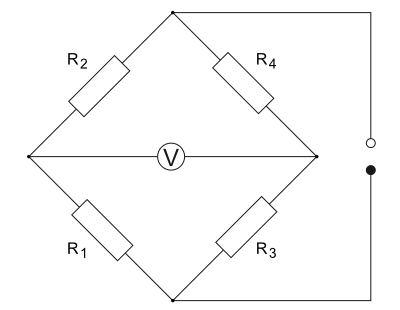
\includegraphics[scale=0.8]{schaltung.png}
\caption{\label{img:schaltung}Aufbau der Wheatstoneschen Brückenschaltung\protect\footnotemark}
\end{figure}
\footnotetext{https://lp.uni-goettingen.de/get/text/3665}

\section{Durchführung}
\label{sec:durchfuehrung}



\section{Auswertung}
\label{sec:auswertung}



\section{Diskussion}
\label{sec:diskussion}

\end{document}
